\subsection{Architectural Views}

\subsubsection{Logical View} % which is the object model of the design, end-user functionality (Class diagrams)
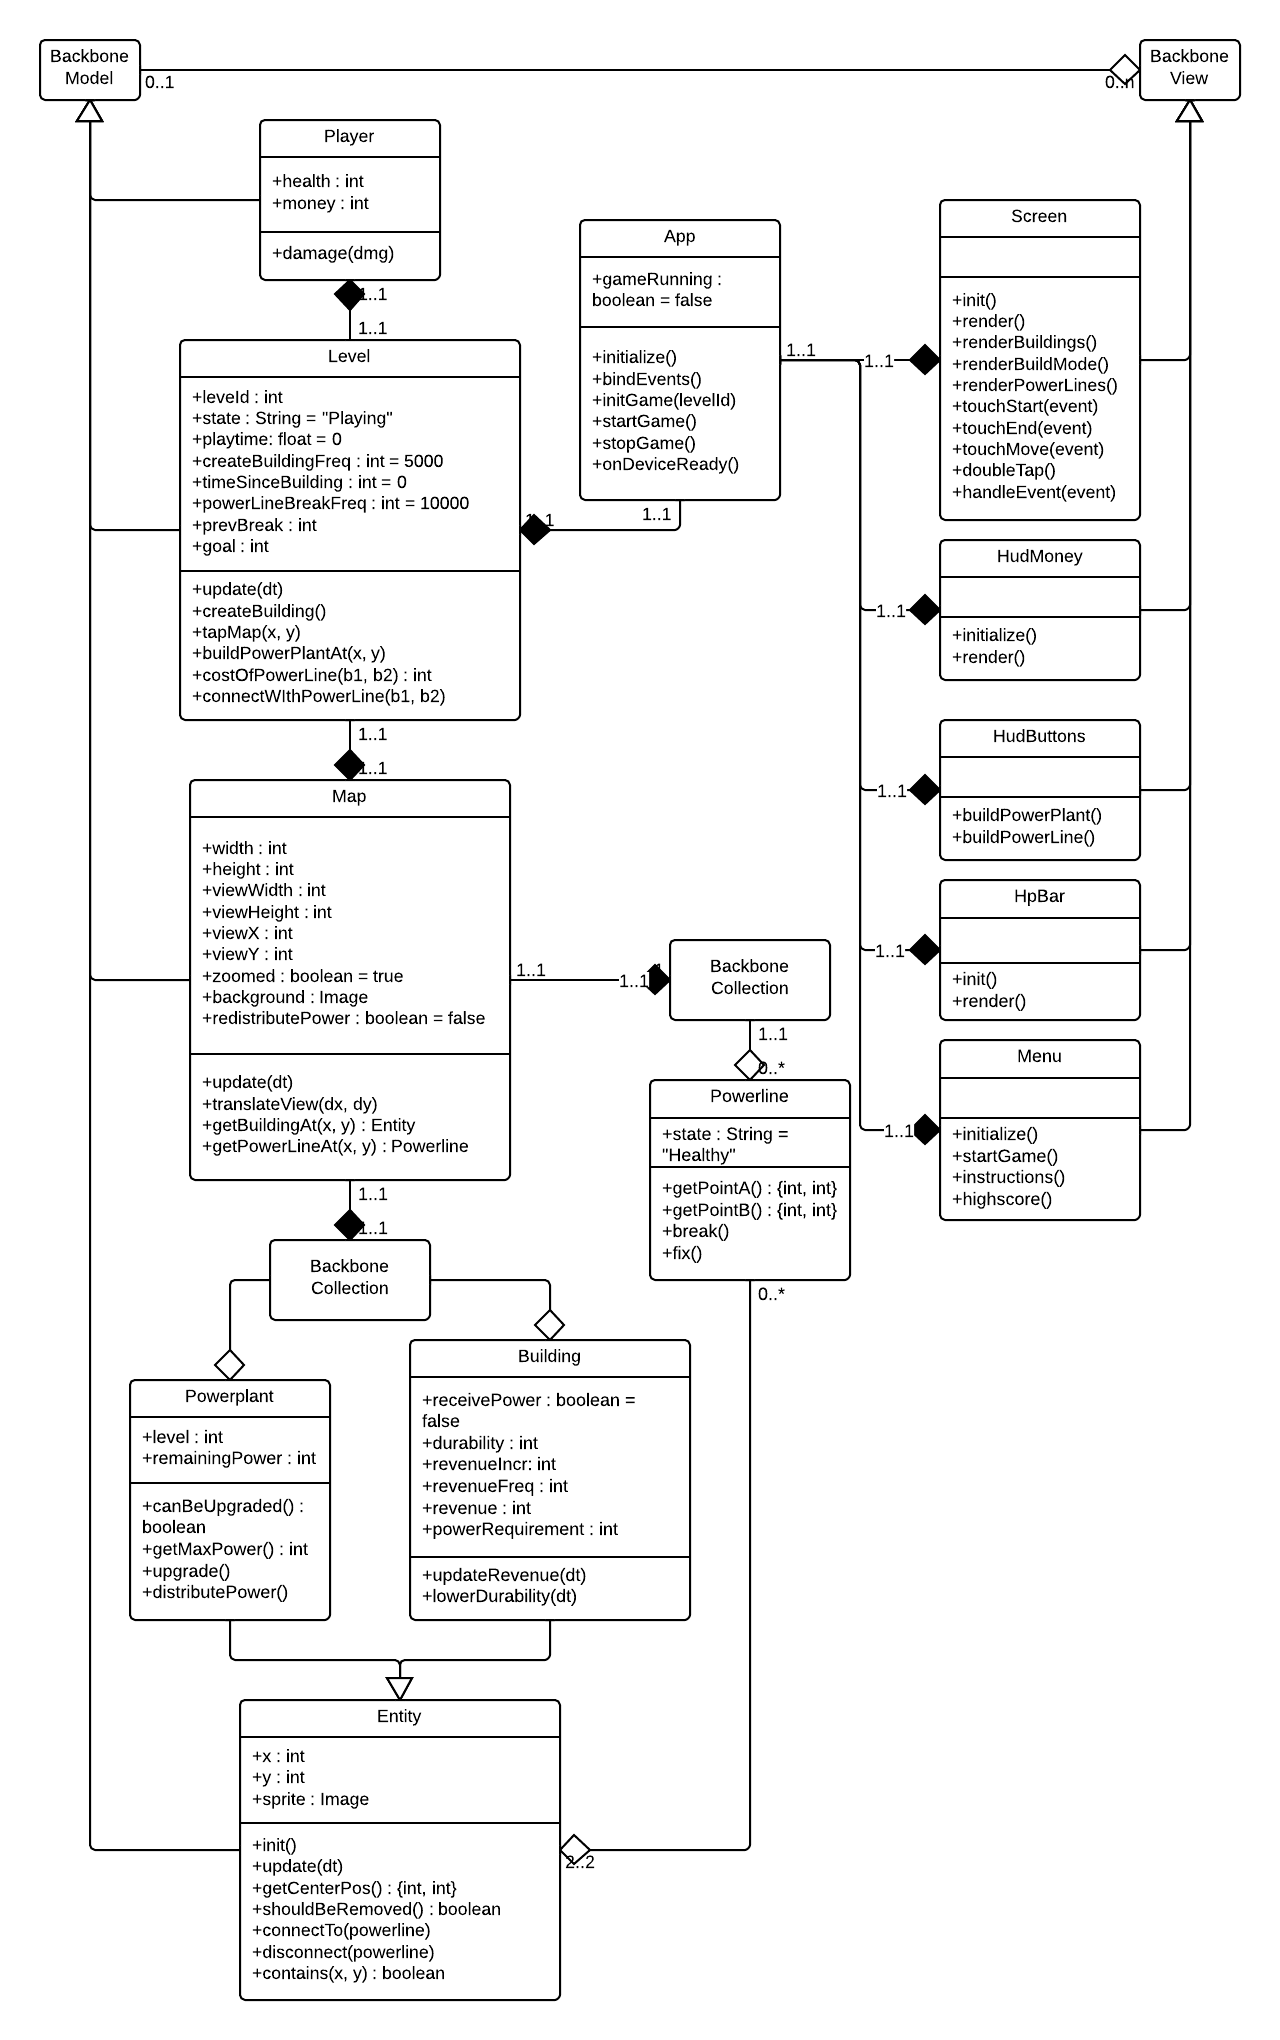
\includegraphics{/pictures/class_diagram.png}

\subsubsection{Process View} % captures the concurrency and synchronization aspects of the design, itegrators, performance, scalability. Takes into account some non-functional requirements, like performance and reliability.

\subsubsection{Physical View} % describes the mappings of the software onto the hardware, and reflects its distributed aspect, system engineers, topology, communications

\subsubsection{Development View} % describes the static organization of the software in its development environment, programmers, software management

\subsubsection{Scenarios} % Bla bla bla, and the illustrated by a few selected use cases, or scenarios which becomes a fifth view
